\documentclass[oneside,fontset=founder]{ctexbook}

\usepackage{geometry}% 用于页面设置
\usepackage[dvipsnames, svgnames, x11names]{xcolor}% 颜色支持
\usepackage{graphicx}% 图形支持
\usepackage[
  colorlinks=true,
  linkcolor=Navy,
  urlcolor=Navy,
  citecolor=Navy,
  anchorcolor=Navy
]{hyperref}% 设置超链接颜色
\usepackage{enumerate}% 枚举支持
\usepackage{minted}% 代码显示支持

% 纸张设置
\geometry{
  b5paper,
  left = 1in,
  right = 1in,
  top = 1in,
  bottom = 1in
}

% 设置章节标题左对齐,+=表示在原有格式上追加,如果只有=则表示完全替换
\ctexset{
  chapter/format += \raggedright,
  section/format += \raggedright,
  subsection/format += \raggedright,
  subsubsection/format += \raggedright,
}

\emergencystretch = \maxdimen% 断字处理
\setlength{\parindent}{2em}% 缩进
\setlength{\parskip}{1ex} % 段间距

% 定义颜色
% \definecolor{pageYellow}{HTML}{F2F1D7}

% \pagecolor{pageYellow}


% ------------------ 开始 -------------------


\begin{document}


% ------------------ 封面 -------------------
\begin{titlepage}%
\begin{center}
  \quad

  \vspace{2ex}

  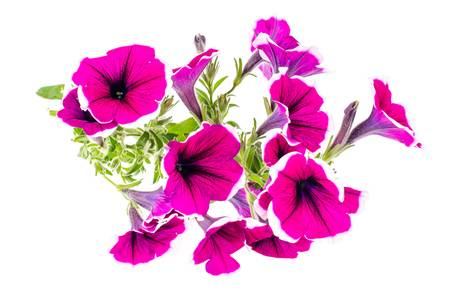
\includegraphics[width=.4\textwidth]{images/cover.png}

  \vspace{4ex}

  \Huge\heiti Petunia项目开发记录\normalsize\normalfont

  \vspace{4ex}

  陆巍
  \vfill%
  % Bottom of the page
  2023年10月5日
\end{center}
\end{titlepage}


% ------------------ 前言 -------------------
\frontmatter% 关闭章节序号,页码使用罗马数字


\chapter{前言}



% ------------------ 目录 -------------------
\tableofcontents% 生成目录


% ------------------ 正文 -------------------
\mainmatter

\chapter{词法分析}


\section{状态转换图}


\subsection{注释}
\begin{tikzpicture}[node distance=9em]
  \node[state,initial]    (s101)               {$101$};
  \node[state]            (s102)[right=of s101]{$102$};
  \node[state, accepting] (s103)[right=of s102]{$103$};
  \path[->](s101) edge [loop above] node {space, $\backslash$t, $\backslash$n, $\backslash$r} ()
                 edge node [above] {\#} (s102)
           (s102) edge [loop above] node[text width=12em, align=center] {characters containing tabs but no other control characters($\backslash$0x00$\sim\backslash$0x08, $\backslash$ 0x0A$\sim\backslash$0x1F, $\backslash$0x7F)} ()
                  edge node[above] {$\backslash$n} (s103);
\end{tikzpicture}


\chapter{开发日记}


\section{2023年10月}


\subsection{10月5日}
这个项目最初只是打算使用简单的判断方法来解决,但想到以后要开发其他编译器,所以先用这个微小项目来练练手。项目将按照编译器开发方法来实现,当然,本项目过于微小,大概只会用到词法分析与语法分析。

Windows系统和Linux系统在文本处理上是有些差异的,其中的换行就不相同。Windows系统中的换行实际上包含了两个字符,即$\backslash r$(回车,0xD)与$\backslash n$(换行,0xA),而Linux系统中只有$\backslash n$(换行,0xA)。我现在主要使用的是Linux系统,但为了兼顾Windows系统,可能需要在读入配置文件后,先把其中的$\backslash r\backslash n$替换成$\backslash n$,然后才做词法分析。

目前暂时只解析裸键名,引号键名以后再考虑。


\subsection{10月6日}
在绘制状态转换图时,我们看到在识别某些内容时,可以按照不同的权衡有不同的处理方式。例如在判断整数时,可以在出现非数字符号就截止,也可以规定必须要出现空格、换行符或\#才截止,两种方式一个宽松,一个严格,各有各的好处与不足。前一种方式对TOML的书写格式比较宽松,但也因为过于宽松可能导致混乱,并增加后期处理的负担。后一种方式要求严格,书写时会有更多约束,但可以减少后期处理的工作量。这里说的后期处理主要是指语法分析阶段。


\subsubsection{10月7日}
随着状态转移图绘制的深入,会让人感到越来越繁琐,或许应该创建一个专门的工具来绘制,并且在绘制完成后自动转换成相应表格直接供词法分析器调用。这个工具的原理并不复杂,麻烦的是图形操作方面的支持问题,这将涉及到图形库方面,这是一个老话题了,先放一放。


\subsection{10月12日}
绘制状态转换图时,我曾经想到对于不合法的符号要如何在图中去处理,这是一种流程图的思维习惯。实际上,在状态转换图中并不需要显式指明如何处理不合法的符号,而是已经暗含了处理方式。合法的符号串可以从状态转换图的开始(start)处走到某一个终点,不合法的符号是没有路径的,在程序处理上会自动跳到错误处理模块,通常会向用户报告某行某列出现词法错误。通常情况下,每发现一个错误就退出程序并报告此错误,也可以把每一行视为一个单元,全部扫描后统一报告。全部扫描的方式还有一些细节问题需要考虑,并非简单的逐行处理就可以。

在把状态转换图映射为状态转换表时,需要把使用到的符号、状态都列出来,这项工作的繁琐程度会随着语言的复杂程度的增加而增加。对于本项目,即使只是简化版的,其状态转换图已经有些繁琐。


\section{2023年11月}


\subsection{11月13日}
在绘制状态转换图时,对于各个状态的编号,一开始我会习惯性的从1开始顺序编写。这样做对于后面的修改并不方便,因为每次修改中间的编号都要对后续的编号重新编写。因此,现在改为使用分段编号,例如注释是100开头,祼键使用200开头。这种方法就需要在状态转换表中增加一列参数来标明编号,以取代原来隐含的自然顺序编号。在实际的程序处理中,会多出一些用于判断编号的代码,虽然会增加一点开销,但有利于设计。

原本我打算在LibreOffice Draw中用一张图来完整描绘状态转换图,但发现这张图越来越大,不利于观看,因此将其拆分为各段,并使用LaTeX的tikz宏包来绘制。虽然也可以在LibreOffice Draw中分页绘制,但为了方便本记录的查阅,就还是放在LaTeX中吧。


\subsection{11月16日}
原来的状态转换图中,无意中把数组用词法分析的形式画上去了,这实际上是不对的,正确的情况应该只是有数组中使用的定界符,即左右中括号。


\subsection{11月18日}
当编写状态转换表时,会面临以何种方式来实现的问题。最简单的方法是把这个表直接放在程序中,使用一个数组来保存,但这样做不灵活,因为每次修改都需要重新编译程序。如果我们把这个表用CSV格式存放在外部的话,灵活性确实有了,但增加了对这个表进行解析的工作。我们不能指望存放这张表的文件中全部是文本字符,应该考虑其中可能包含非文本字符的情况,因此从更通用的角度出发,需要引入转义字符的方式来可视的实现此表的编辑。毕竟不可见的符号编辑时需要使用二进制编辑工具来处理,不直观。这里我将按照C语言中转义字符的使用规则来处理,会在程序中添加一套词法解析的代码,只不过这个词法解析代码的规则将直接写在程序中,不再以外部文件的形式存放。

至此,我们可以看到,这个小项目中出现了两个词法解析,一个用于解析TOML配置文件,一个用于解析TOML的词法规则文件。


\subsection{11月21日}
使用CSV格式来保存状态转换关系,还是存在一些符号方面的问题。通常情况下,CSV分隔数据使用的是逗号,那么如果数据中包含逗号,那就需要做转义处理,一般是使用双引号。这样做感觉还是不算用户友好,所以我计划使用SQLite这一轻量级数据库来保存状态转换表。使用SQLite自然需要增加一些开销,包括引入相关源码文件和数据库管理工具,目前看来是可以接受的。这个就是数据符号与格式符号的混淆问题。

对于状态转换表中的实际内容,并不象我们绘制的图形中那样,让人想到的是一个一个的字符判断语句,具体的处理方法是使用正则表达式的规则字符串来实现。这样做可以实现通用性。例如,我们在判断一个字符是否属于字母时,一般的C语言代码中可以使用ASCII码的数值比较来判断,但这样做实际上就把规则固化在程序中,以后做调整时需要修改程序。使用正则表达式的规则字符串的话,就把程序与具体的转换规则彻底分离,以后的规则调整不再需要修改程序重新编译了。不管是什么规则,在程序中都只是简单的与内容无关的一个判断语句。



\end{document}